Algorithms \ref{alg:p1alg1} and \ref{alg:p1alg2} can be used for fast optimisation of magnetic systems. Presented here is one such case, wherein two pyramidal frustums are arranged with magnet B above magnet A, as shown in Figure \ref{fig:p1frustumcase}. Both magnets have a unit magnetisation strength of 1 Tesla. The magnetisation vectors are oppositely directed with the magnets in repulsion. The wall angle \(\theta\) is varied to maximise the force at a given distance while the magnet height and volume are kept constant at 5cm and 500cm\(^3\) respectively. A wall angle of \(\theta = 90^\circ\) corresponds to a cuboidal magnet with a height of 5cm and both width and depth of 10cm.
\begin{figure*}
	\centering
	\begin{subfigure}{0.4\textwidth}
		\centering
		\tdplotsetmaincoords{70}{110}
		\begin{tikzpicture}[scale=40,tdplot_main_coords]
		\coordinate(p1t) at (-0.050000,-0.050000,-0.000000);
		\coordinate(p2t) at (-0.050000,0.050000,-0.000000);
		\coordinate(p3t) at (0.050000,-0.050000,-0.000000);
		\coordinate(p4t) at (0.050000,0.050000,-0.000000);
		\coordinate(p5t) at (-0.025000,-0.025000,0.050000);
		\coordinate(p6t) at (0.025000,-0.025000,0.050000);
		\coordinate(p7t) at (-0.025000,0.025000,0.050000);
		\coordinate(p8t) at (0.025000,0.025000,0.050000);
		
		\coordinate(p1b) at (0.050000,0.050000,-0.025000);
		\coordinate(p2b) at (0.050000,-0.050000,-0.025000);
		\coordinate(p3b) at (-0.050000,0.050000,-0.025000);
		\coordinate(p4b) at (-0.050000,-0.050000,-0.025000);
		\coordinate(p5b) at (0.025000,0.025000,-0.075000);
		\coordinate(p6b) at (-0.025000,0.025000,-0.075000);
		\coordinate(p7b) at (0.025000,-0.025000,-0.075000);
		\coordinate(p8b) at (-0.025000,-0.025000,-0.075000);
		
		\draw[fill=white] (p4b) -- (p3b) -- (p1b) -- (p2b) -- cycle;
		\draw[fill=white] (p1b) -- (p3b) -- (p6b) -- (p5b) -- cycle;
		\draw[fill=white] (p1b) -- (p2b) -- (p7b) -- (p5b) -- cycle;
		
		\draw[fill=white] (p5t) -- (p6t) -- (p8t) -- (p7t) -- cycle;
		\draw[fill=white] (p2t) -- (p4t) -- (p8t) -- (p7t) -- cycle;
		\draw[fill=white] (p6t) -- (p8t) -- (p4t) -- (p3t) -- cycle;
		
		\node(A) at (-0.0375,-0.025,-0.08) {\text{A}};
		\node(B) at (-0.0375,-0.025,-0.005) {\text{B}};
		\end{tikzpicture}
		\caption{}
	\end{subfigure}
	~ \hspace{20pt}
	\begin{subfigure}{0.4\textwidth}
		\centering
		\tdplotsetmaincoords{90}{0}
		\begin{tikzpicture}[scale=40,tdplot_main_coords]
		\coordinate(p1t) at (-0.050000,-0.050000,-0.000000);
		\coordinate(p2t) at (-0.050000,0.050000,-0.000000);
		\coordinate(p3t) at (0.050000,-0.050000,-0.000000);
		\coordinate(p4t) at (0.050000,0.050000,-0.000000);
		\coordinate(p5t) at (-0.025000,-0.025000,0.050000);
		\coordinate(p6t) at (0.025000,-0.025000,0.050000);
		\coordinate(p7t) at (-0.025000,0.025000,0.050000);
		\coordinate(p8t) at (0.025000,0.025000,0.050000);
		
		\coordinate(p1b) at (0.050000,0.050000,-0.025000);
		\coordinate(p2b) at (0.050000,-0.050000,-0.025000);
		\coordinate(p3b) at (-0.050000,0.050000,-0.025000);
		\coordinate(p4b) at (-0.050000,-0.050000,-0.025000);
		\coordinate(p5b) at (0.025000,0.025000,-0.075000);
		\coordinate(p6b) at (-0.025000,0.025000,-0.075000);
		\coordinate(p7b) at (0.025000,-0.025000,-0.075000);
		\coordinate(p8b) at (-0.025000,-0.025000,-0.075000);
		
		\draw[gray] (p2b) -- (p4b) -- (p8b) -- (p7b) -- cycle;
		\draw[gray] (p1t) -- (p3t) -- (p6t) -- (p5t) -- cycle;
		
		\draw[<->] (0,0,-0.025) -- (0,0,0);
		\node (d) at (0.005,0,-0.0125) {\(d\)};
		
		\draw[->,thick] (0,0,0.035) -- (0,0,0.015);
		\node (M1) at (-0.0075,0,0.025) {\textbf{M}};
		\draw[->,thick] (0,0,-0.06) -- (0,0,-0.04);
		\node (M2) at (-0.0075,0,-0.05) {\textbf{M}};
		
		\node(theta1) at (-0.022,0,0.043){\(\theta\)};
		\node(theta2) at (-0.022,0,-0.068){\(\theta\)};
		\node(A) at (0.025,0,-0.05) {\text{A}};
		\node(B) at (0.025,0,0.025) {\text{B}};
		
		\end{tikzpicture}
		\caption{}
	\end{subfigure}
	\caption{Three-dimensional view (a) and side view (b) of two pyramidal frustum magnets with opposing vertical magnetisations \(\mathbf{M}\). Magnet B moves a distance \(d\) in the vertical direction. The wall angle \(\theta\) is varied while maintaining a constant magnet volume and height.}
	\label{fig:p1frustumcase}
\end{figure*}

The frustums were separated by a given distance \(d\) and the wall angle \(\theta\) varied. For all values of \(\theta\), the repulsive force between the magnets was calculated and divided by the maximum force for each separation to give the normalised force plot shown in Figure \ref{fig:p1frustumforce}. The peaks of this plot correspond to the maximum force at a given separation distance, and hence show the optimal wall angle for that distance. The optimal angle was calculated for several separation distances using this method with the results shown in Table \ref{tab:p1optimalfrustum}. It can be seen that the optimal wall angle increases with separation distance, indicating that as the magnets move further apart, the optimal shape tends toward a pyramid. On the contrary, as the magnets become closer, the optimal shape tends toward a cuboid.
\begin{figure}
	\centering
	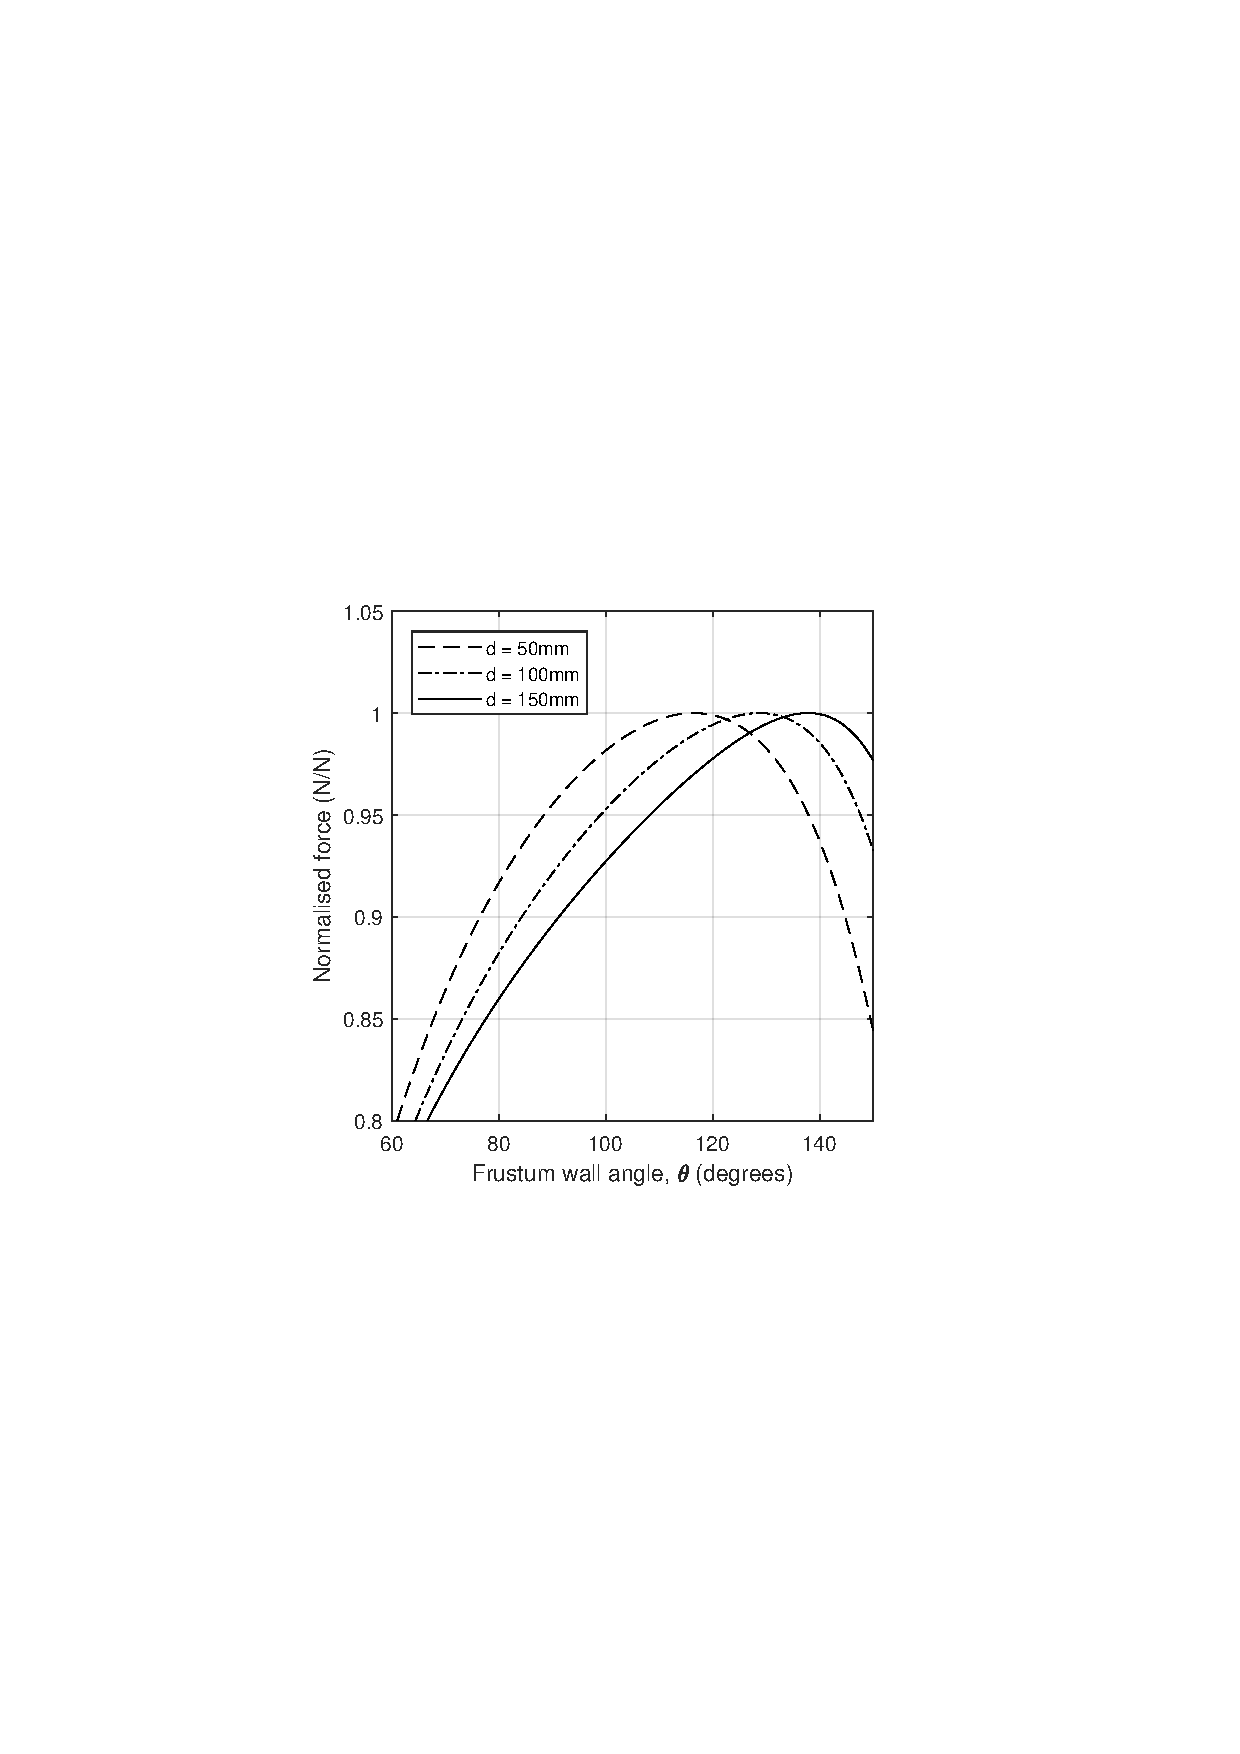
\includegraphics[trim = 5cm 9cm 5cm 9cm,width=0.8\linewidth]{p1/p1FIG8}
	\caption{The normalised force between the two frustum magnets shown in Figure \ref{fig:p1frustumcase} as the wall angle \(\theta\) is varied. Each plot corresponds to a given separation distance \(d\) shown in the legend. The normalised force is calculated by dividing the force at each point by the maximum force for each separation distance. The peak of each plot corresponds to the maximum force attained, and thus the optimal wall angle. As the separation distance increases, the peak moves to the right, indicating the optimum wall angle increases with the separation distance.}
	\label{fig:p1frustumforce}
\end{figure}
\begin{table}
	\centering
	\caption{The optimal wall angle of the pyramidal frustums at a given distance. This angle maximises the repulsive force between the magnets while maintaining a constant magnet volume and height.}
	\begin{tabular}{cc}
		\hline
		Separation distance (mm) & Optimal angle (degrees) \\
		\hline
		25 & 110 \\
		50 & 117 \\
		75 & 123 \\
		100 & 129 \\
		125 & 134 \\
		150 & 138 \\
		\hline
		\label{tab:p1optimalfrustum}
	\end{tabular}
\end{table}

The above test lead to an investigation on optimal angle for a varying separation distance. For a given separation distance, a golden ratio search was implemented to find the optimal angle which maximises the repulsive force. This was repeated for a large range of separation distances, and the plot shown in Figure \ref{fig:p1optimalfrustum} (left) was obtained. Again, it can be seen that the optimal angle increases with the separation distance. Interestingly, when the separation distance is zero, the optimal angle is not 90\(^\circ\). Namely, the optimal geometry is not cuboidal when the magnets are touching. Furthermore, the optimal angle is always greater than 90\(^\circ\), implying that cuboidal magnets are not the optimal geometry for this particular configuration.
\begin{figure*}
	\centering
	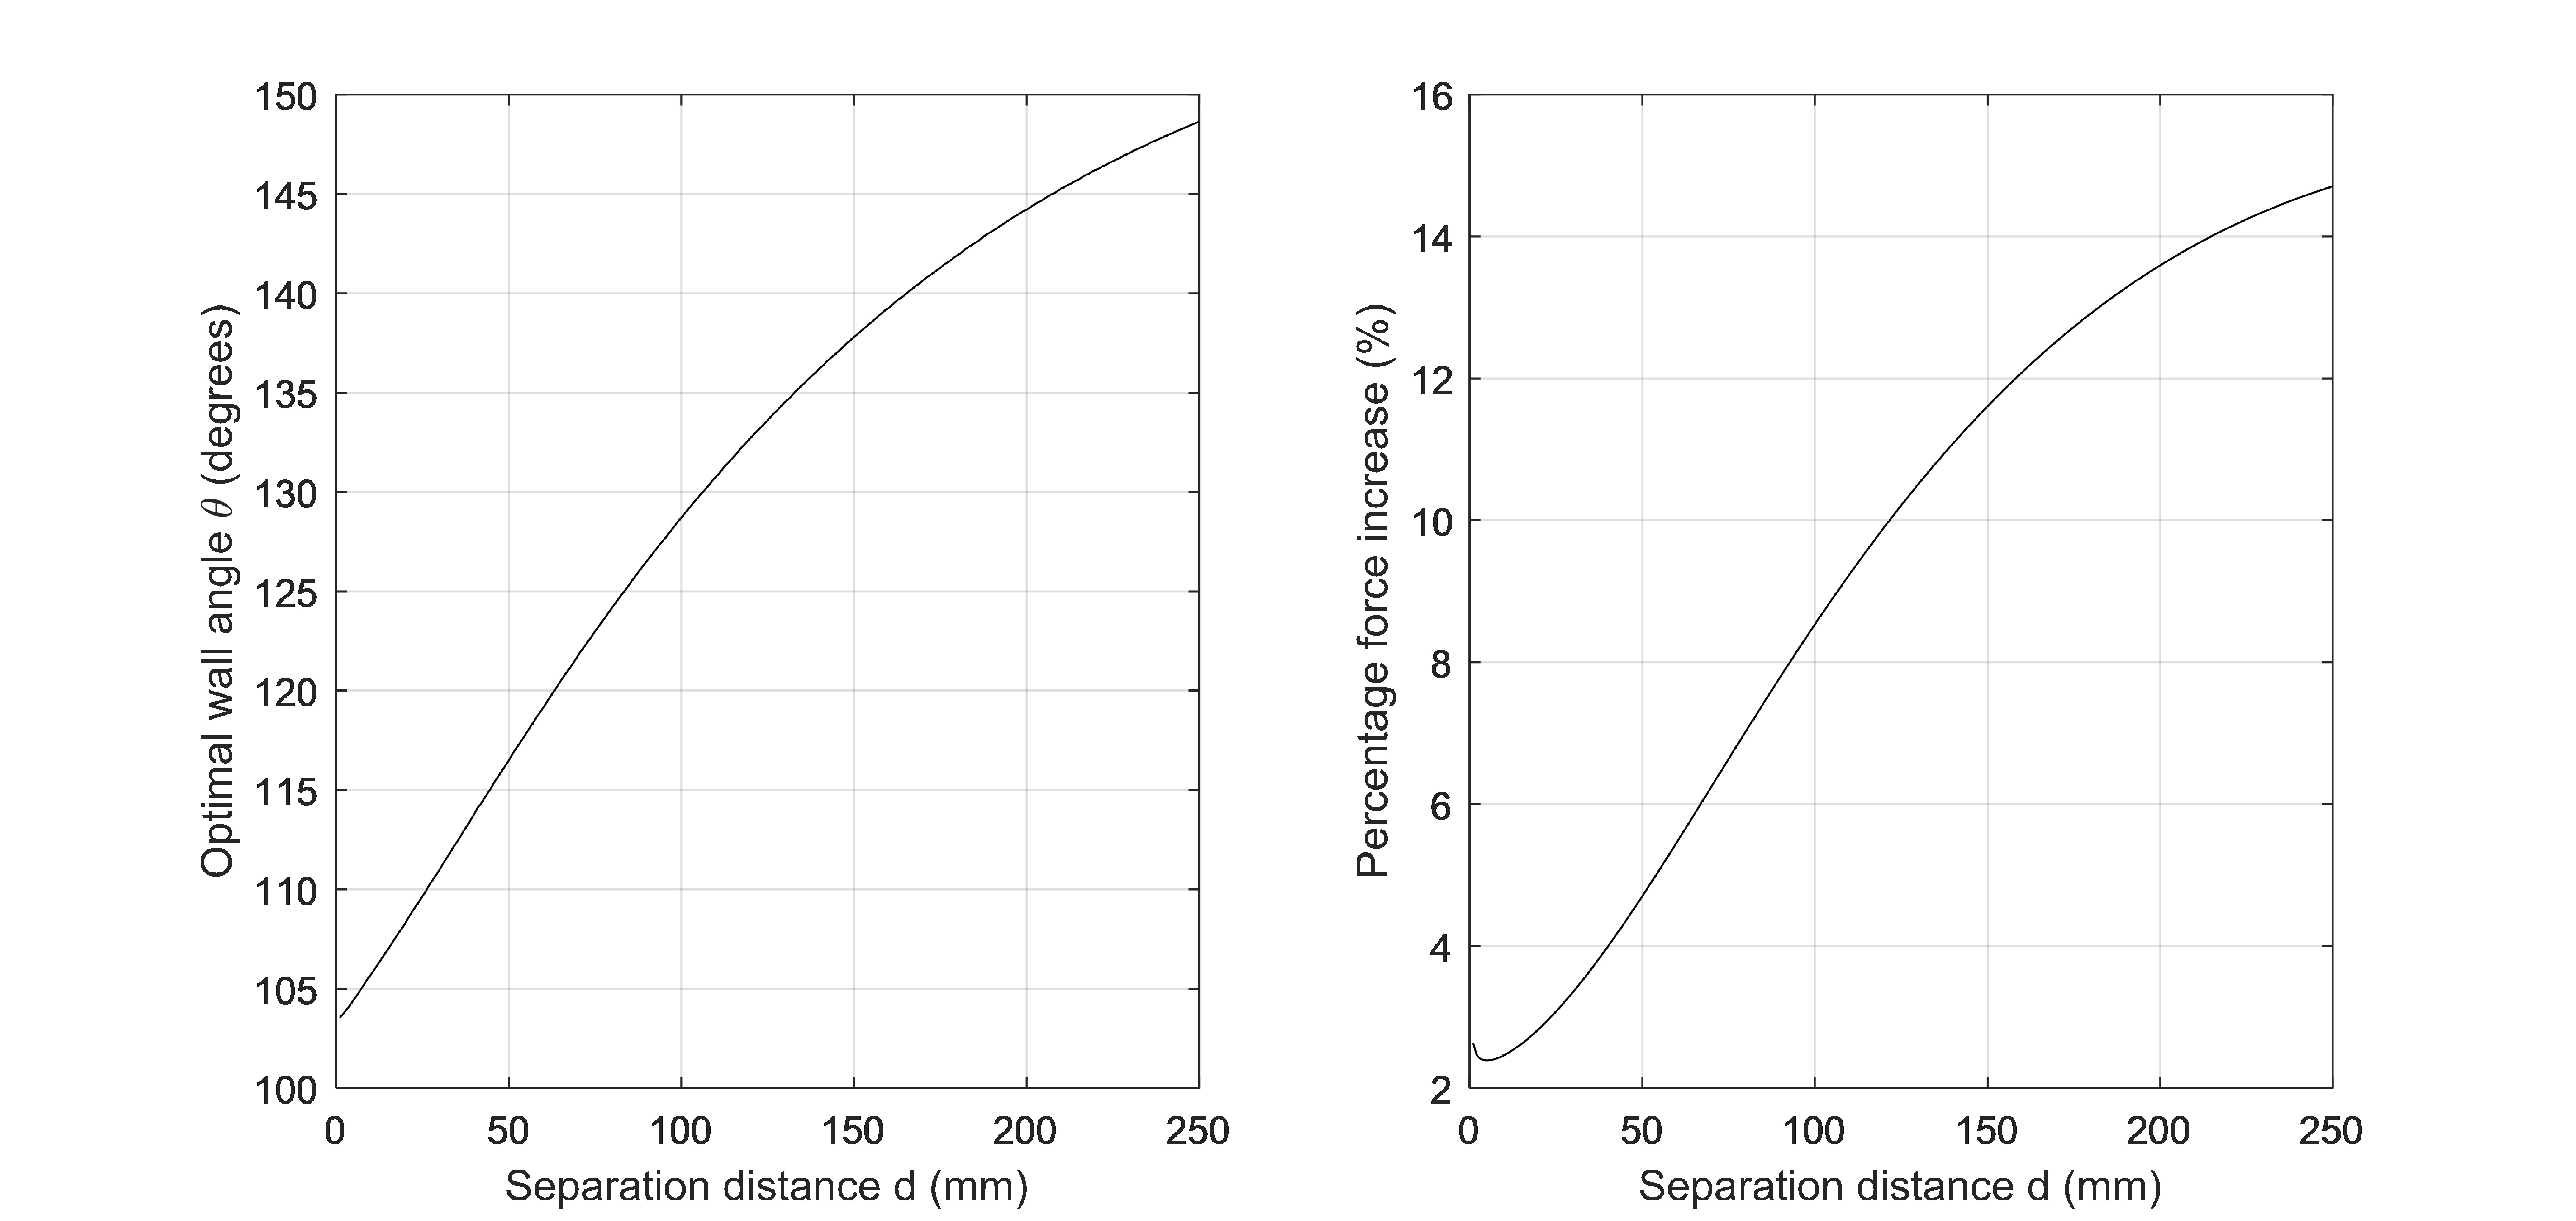
\includegraphics[trim = 4cm 0cm 4cm 0cm,width=\linewidth]{p1/p1FIG9}
	\caption{The optimal wall angle \(\theta\) of the frustums at a given distance to maximise the repulsive force between them (left). At all separation distances, the optimal angle is larger than 90\(^\circ\), indicating a cuboid is never the optimal geometry in this case. The optimal angle increases with separation distance, and tends toward a pyramid geometry at large separations. These results were compared to two cuboidal magnets with equal volume and height at the same separation distances. The force increase as a percentage of the repulsive force between the cuboids was found (right). A considerable increase in force was found, especially at larger separations. This implies that a larger force can be achieved with smaller mass if the system is optimised.}
	\label{fig:p1optimalfrustum}
\end{figure*}

In addition to calculating the optimal angle at a given separation distance, the percentage force increase was calculated. For each separation distance, the maximum force was found, as well as the force between two cuboidal magnets of equivalent height and volume. The percentage force increase is defined as
\begin{equation}
\text{PFI} = \frac{F_\text{frustum}-F_\text{cuboid}}{F_\text{cuboid}} \times 100\% \text{.}
\end{equation}
This percentage force increase was plotted against separation distance (Figure \ref{fig:p1optimalfrustum}, right). This value increases with separation distance, corresponding to a larger wall angle. Additionally, the force increase is positive for all separation distances, meaning with a constant magnetic volume, polyhedral magnets can achieve larger forces than cuboidal magnets. Alternatively, the same forces can be achieved using a smaller system mass, which could lead to significant cost savings.